\chapter{IMPLEMENTATION}


% (20\% of Report Length)

% a. Showcase the output at various intermediate stages of the project pipeline

% b. Use proper data visualizing techniques to present the output

% c. Figures and tables must be accompanied by an explanation
\section{Tools Used}
\textbf{Figma}\\
Figma is a cloud-based design and prototyping tool that empowers teams to collaborate on UI/UX design projects in real-time. It offers a user-friendly interface and powerful features that make it a popular choice among designers. With Figma, designers can create and share interactive prototypes, design components, and design systems. Its cloud-based nature allows for seamless collaboration, enabling multiple team members to work on the same design simultaneously. Figma supports version control, ensuring that design iterations can be easily tracked and managed. \\
\textbf{React}\\
React is a widely-used open-source JavaScript library developed by Facebook for building user interfaces, particularly single-page applications where data changes frequently. It emphasizes a component-based architecture, allowing developers to create reusable UI components that encapsulate their own structure, logic, and styling. React’s use of a virtual DOM enhances performance by minimizing direct updates to the real DOM, ensuring efficient rendering. With its declarative approach, developers specify what the UI should look like based on different states, making the code more predictable and easier to debug. Additionally, React introduces JSX, a syntax extension that combines JavaScript and HTML, making it straightforward to write and understand UI components.\\
\textbf{Postgres}\\
PostgreSQL, often referred to simply as Postgres, is a powerful open-source relational database management system known for its reliability, robustness, and extensibility. Developed over decades and maintained by a global community of contributors, PostgreSQL offers a comprehensive set of features for managing structured data. It supports complex queries, transactions with ACID (Atomicity, Consistency, Isolation, Durability) properties, and a wide range of data types including JSON, XML, and spatial data. PostgreSQL's commitment to standards compliance and continuous improvement ensures compatibility with various programming languages and frameworks. With capabilities for scalability, data integrity, and advanced indexing, PostgreSQL is a preferred choice for applications requiring robust data management and high availability, contributing to its widespread adoption aweb industries from small startups to large enterprises. \\
\textbf{Git/Github}\\
Git is a distributed version control system that is both free and open-source, designed to handle projects of all sizes efficiently and swiftly. It simplifies collaboration by enabling multiple individuals to contribute changes that can be seamlessly merged into a single source. When using Git, the software runs locally on your computer, storing your files and their complete history. Alternatively, you can utilize online hosts like GitHub to store a copy of your files and their revision history. This central repository allows you to easily upload your changes and download updates from other developers, promoting seamless collaboration. Git facilitates automatic merging of changes, allowing multiple individuals to work on different sections of the same file and later merge their modifications without losing any work.\\
\textbf{Node Js with Express}\\
Node.js with Express.js is a powerful combination for building scalable and efficient web applications. Node.js provides a runtime environment that allows JavaScript to be executed server-side, leveraging its event-driven, non-blocking I/O model to handle multiple concurrent connections efficiently. Express.js, as a minimalist web framework for Node.js, simplifies the creation of APIs and routes, offering robust features such as middleware support, routing, and template engines. Together, Node.js and Express.js enable rapid development of RESTful APIs and web servers, making them well-suited for creating real-time applications, microservices, and backend systems. With a vibrant ecosystem of libraries and active community support, Node.js with Express.js remains a popular choice for developers seeking flexibility, performance, and scalability in web application development.\\
\textbf{JavaScript}\\
JavaScript is a programming language that is used to create interactive web pages and backend server. It is a powerful and versatile language that can be used to do a wide variety of things, including adding animation and interactivity to web pages, validating form data, processing user input, making Ajax requests to the server, and creating games and other interactive applications.\\
\textbf{Phaser}\\
Phaser is a powerful and popular open-source HTML5 game framework designed for creating 2D games that can run in both web browsers and mobile environments. Developed by Photon Storm, Phaser is known for its versatility and ease of use, making it a favorite among both beginner and experienced game developers. The framework supports Canvas and WebGL rendering, automatically selecting the best option based on the device's capabilities. Phaser offers a robust set of features including physics engines (Arcade Physics, P2 Physics, and Matter.js), input handling, asset management, animations, and audio integration. Its component-based architecture allows developers to build complex games by combining reusable pieces of code, enhancing modularity and maintainability. With an active community, extensive documentation, and numerous tutorials, Phaser provides ample resources for learning and development, empowering creators to bring their game ideas to life efficiently.
\section*{Postman}
Postman is a widely-used collaboration platform for API development, enabling developers to design, test, document, and monitor APIs with ease. Originally starting as a simple Chrome extension, Postman has evolved into a comprehensive tool that supports the entire API lifecycle. Its intuitive interface allows developers to construct and send HTTP requests to interact with APIs, receiving detailed responses to inspect and debug.

\section*{Unity 3D}
Unity 3D is a leading game development platform renowned for its ability to create both 2D and 3D interactive experiences across a wide range of platforms, including consoles, mobile devices, and VR/AR environments. Developed by Unity Technologies, the engine offers a comprehensive suite of tools that cater to every aspect of game development, from design and prototyping to final deployment.
Unity’s real-time rendering capabilities, coupled with its powerful physics engine, allow developers to create highly immersive and visually stunning games. The engine's support for WebGL enables developers to deploy their games directly to the web, providing browser-based experiences without the need for plugins. WebGL in Unity leverages the engine's advanced rendering capabilities, allowing developers to create complex 3D environments that run smoothly in any modern browser. This makes Unity a versatile tool not only for traditional game development but also for creating interactive web applications.
\section*{Draw.io}
Draw.io (now known as diagrams.net) is a powerful, web-based diagramming tool designed to simplify the creation of various types of visual diagrams, including flowcharts, organizational charts, network diagrams, and more. Developed to be user-friendly and accessible, Draw.io provides a comprehensive suite of features that facilitate diagram creation and collaboration. The tool offers a wide range of pre-built templates, shapes, and connectors, allowing users to quickly construct detailed diagrams tailored to their specific needs. With its intuitive drag-and-drop interface, users can easily customize and arrange elements to convey complex information clearly and effectively. Draw.io also integrates seamlessly with cloud storage services like Google Drive and Dropbox, enabling real-time collaboration and ensuring that diagrams are easily accessible from anywhere. Its flexibility and ease of use make it an invaluable resource for professionals and teams seeking to visualize data, plan projects, or streamline workflows.
\section*{Figma}
Figma is a leading web-based design tool renowned for its collaborative capabilities and versatility in creating user interfaces, prototypes, and vector graphics. Developed by Figma, Inc., the platform provides a robust set of design features that support both individual and team-based projects. With real-time collaboration, multiple users can simultaneously work on the same design, offering a seamless experience for brainstorming, feedback, and iterative design processes. Figma’s vector graphics editor allows for precise design work, while its prototyping tools enable users to create interactive and dynamic prototypes that simulate the user experience. The platform supports extensive plugin integrations, enhancing functionality and streamlining workflows. Its cloud-based nature ensures that designs are always up-to-date and accessible from any device, making Figma an essential tool for modern design teams seeking efficient and collaborative design solutions.


\subsection{Implementation Details of Modules}
This subsection outlines the implementation specifics for each module, detailing the core functionalities and algorithms utilized. It covers the programming languages, frameworks, and tools used in development, along with the interaction and communication between modules. Key design patterns, data management strategies, and error-handling mechanisms are discussed to ensure optimal performance. Additionally, security measures and optimizations applied during implementation are highlighted.
\newline
\newpage
\textbf{Module of AtomSimulator}

The AtomSimulator module initializes the `selectedElement` with the first element from the `elements` array and sets up a Phaser game instance with appropriate dimensions and physics. It visualizes the atom by creating the nucleus and electron orbits, updates electron positions based on time, and handles user interactions to update the element and re-render the scene. The Phaser instance is destroyed upon component unmounting to free resources.
\newline
\textbf{Module of CodeEditor}

The CodeEditor module initializes states for `code` and `consoleOutput`. It creates an iframe to execute user-provided JavaScript code and captures console messages and errors. The `consoleOutput` is updated with iframe messages, and the iframe is removed from the DOM after execution to prevent resource leaks.
\newline
\textbf{Module of OhmsLawSimulator}

The OhmsLawSimulator module sets default values for voltage and resistance, initializes a Phaser game instance, and creates game elements. It continuously updates the bulb brightness based on the current \( I = \frac{V}{R} \), adjusts displayed values, and re-renders the simulation with user input changes. The Phaser instance is destroyed on component unmount.
\newline
\textbf{Module of GravitySim}

The GravitySim module sets up a Phaser game environment with gravity simulation. It creates game elements, displays initial values, and updates gravity, distance, and time during the simulation. Users can adjust gravity, reset the player, and pause or resume the simulation. The Phaser instance is destroyed on component unmount. The distance traveled is calculated using \( d = \frac{1}{2} g t^2 \).
\newline
\textbf{Module of SolarSystemSimulator}

The SolarSystemSimulator module initializes celestial bodies and the main camera. It attaches a `RotateAround` script to simulate planetary and moon orbits and a `FollowAtTarget` script to keep the camera focused on the selected object. Users can change the camera target, and the implementation involves creating bodies, configuring camera controls, and testing interactions.
\newpage
\textbf{Frontend API Integration Module}\newline
This diagram depicts the architecture of a web application where a React frontend communicates with an Express server through RTK Query and Axios. The process starts with the React frontend triggering either queries or mutations, which are handled by the Redux Toolkit (RTK) API slices. These slices manage API interactions, including the request and response lifecycle. Axios is used to send HTTP requests from the frontend to the Express server. The server processes incoming requests, performs necessary operations (such as database interactions), and sends responses back to Axios. Axios then passes the response data to RTK slices, which manage state updates. This architecture ensures smooth, organized data flow between the client and server, making it easier to handle API calls, manage state, and ensure a responsive user experience.
\begin{figure}[H]
    \centering
     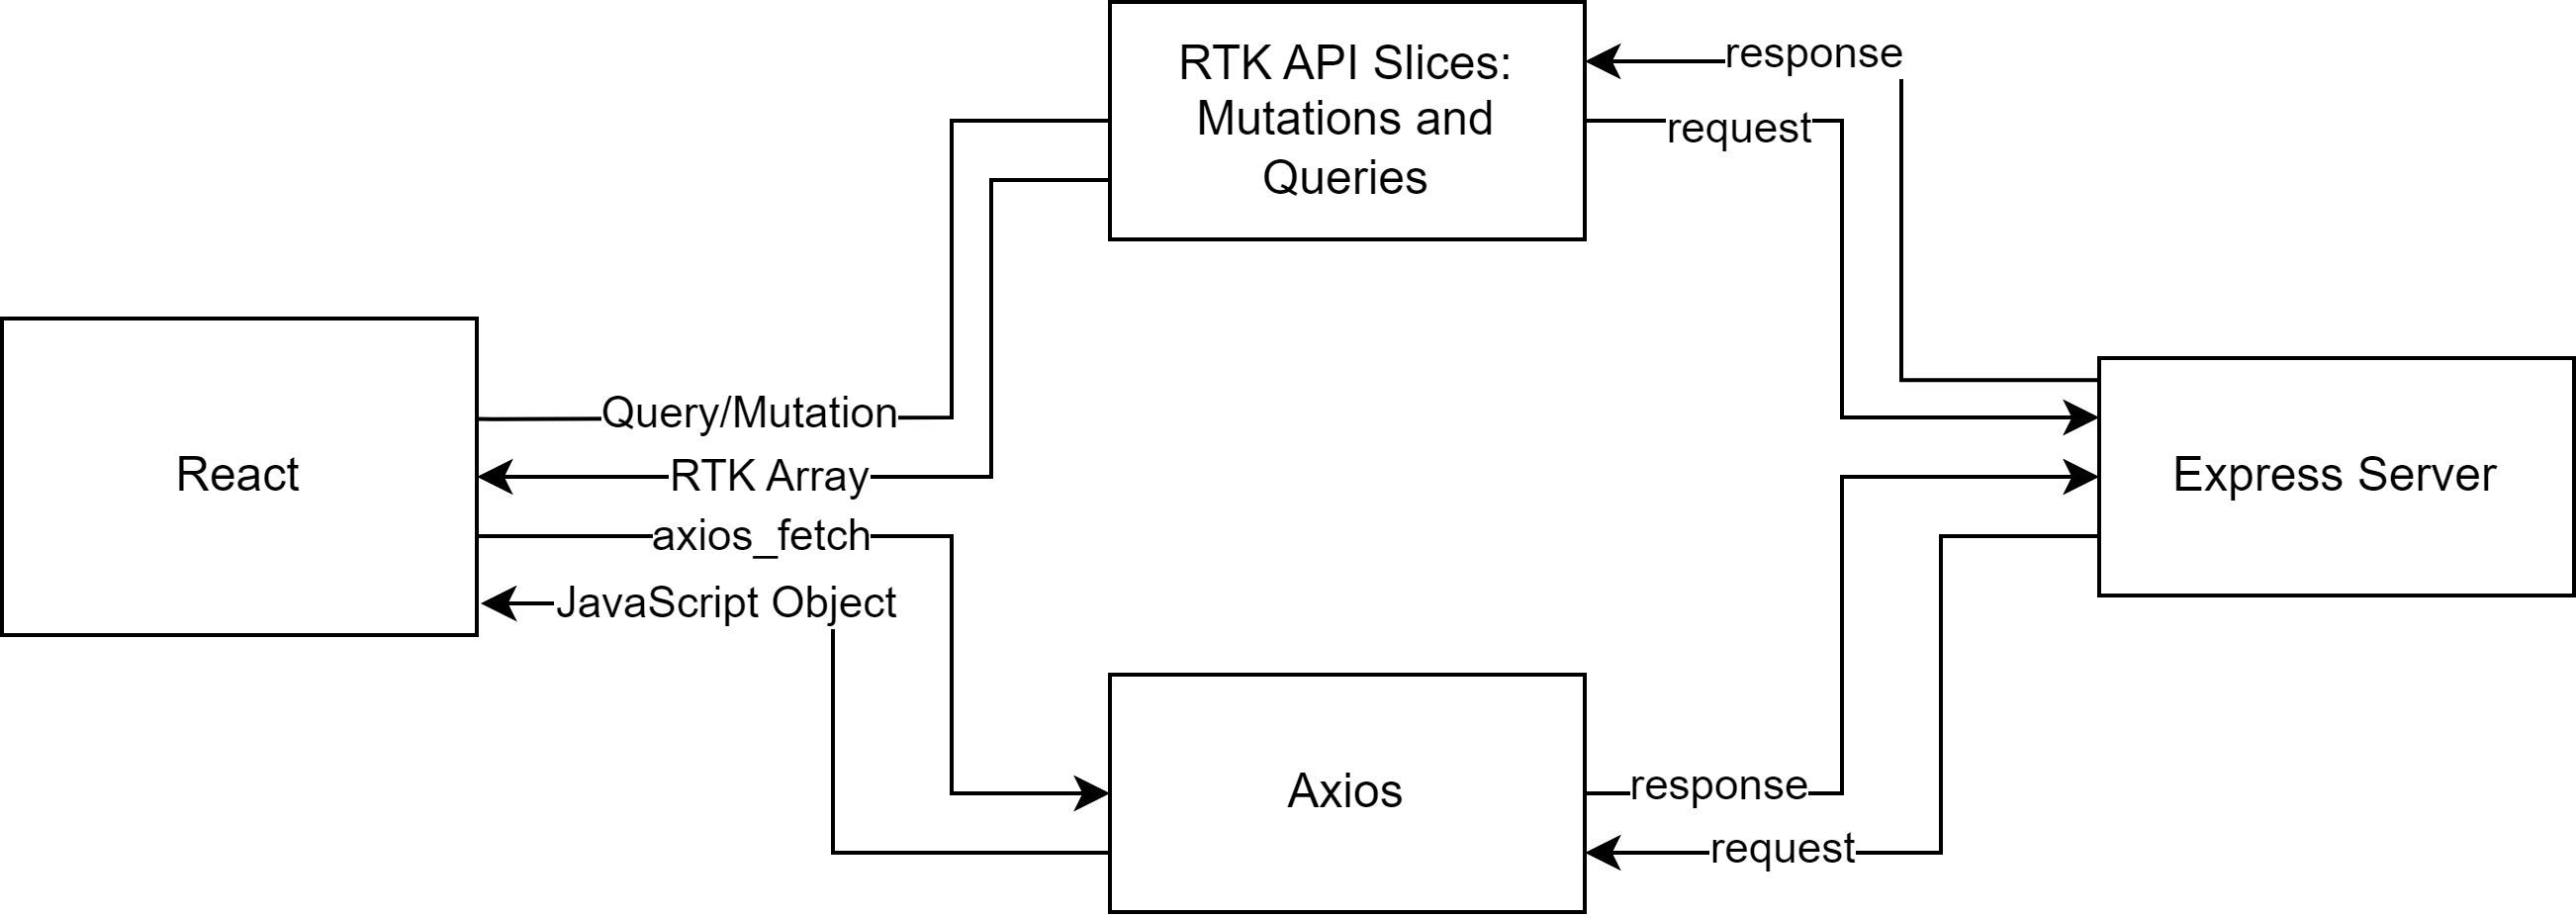
\includegraphics[height = 5cm]{Diagrams/API.png}
     \caption{API Integration Module}
 \end{figure}
\textbf{User Registration Module}

This diagram outlines a registration or authentication process involving several components. The user interacts with a React frontend to register or request access. A Token Generator backend service creates an authentication token, which is sent to the user via email using Node Mailer (implemented with Node.js and Nodemailer). The user submits the token back to the system, and the Token Verification service checks its validity. The Postgres database stores user information and tokens, ensuring that the submitted token matches the one in the database for verification. This flow connects the frontend, backend, email system, and database for user authentication.
\begin{figure}[H]
    \centering
     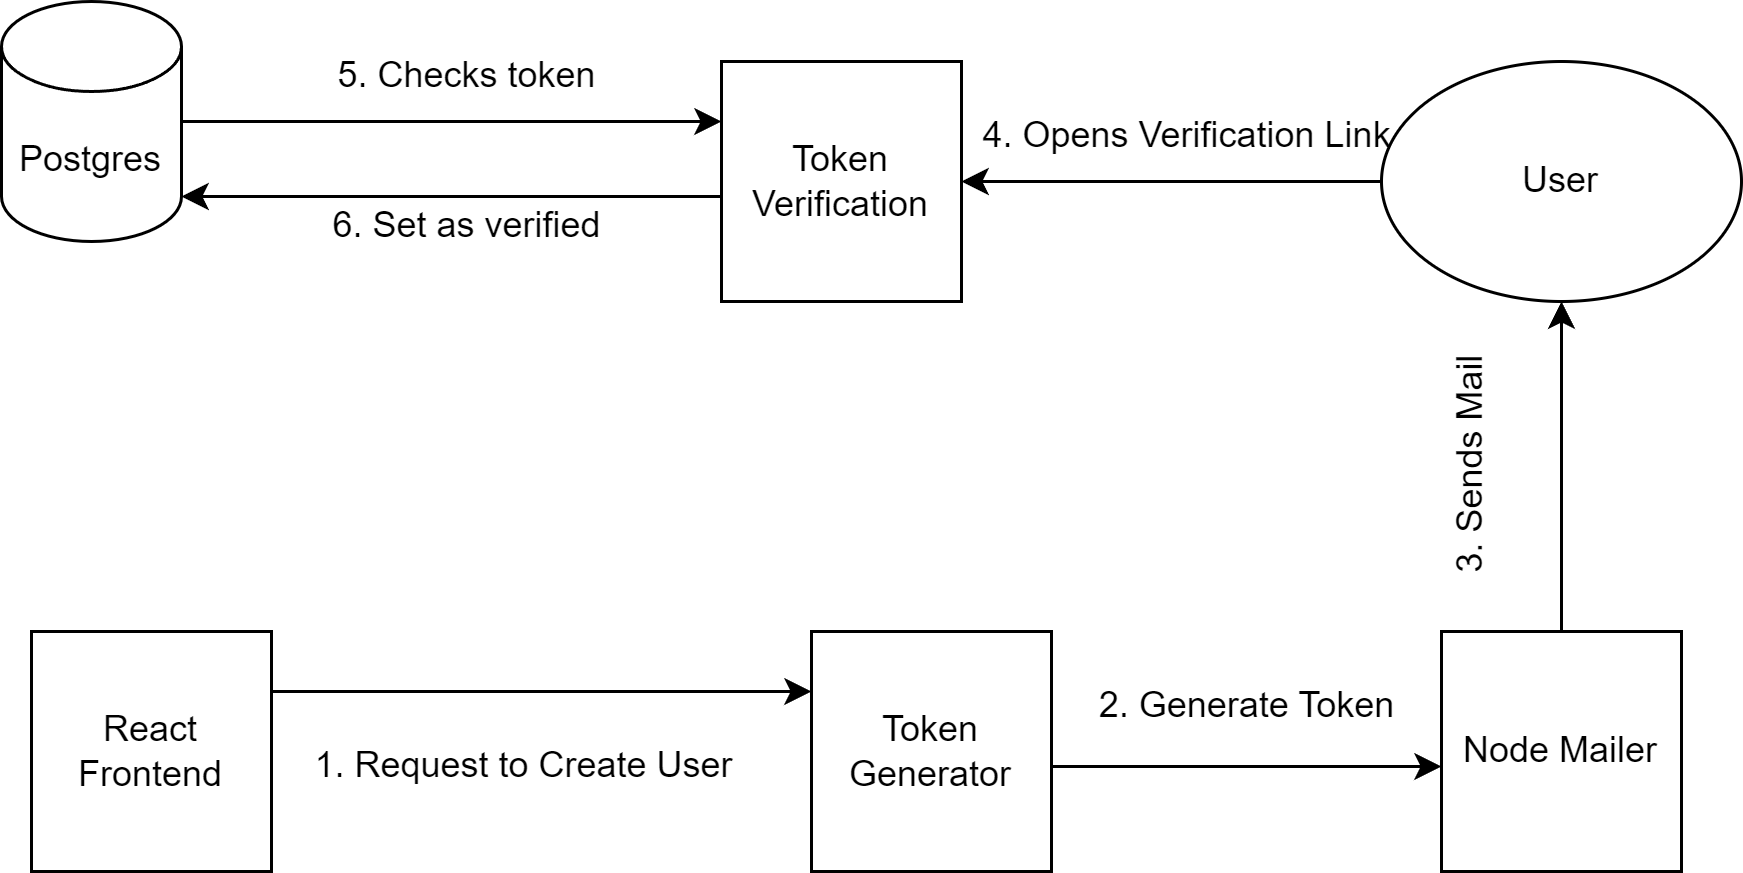
\includegraphics[height = 5cm]{Diagrams/register_module.png}
     \caption{Registration Module}
 \end{figure}
\textbf{Authentication Module}
\newline
The Authentication Module utilizes JSON Web Tokens (JWT) for secure user authentication. JWTs are compact, URL-safe tokens that encode user information, including a signature to verify the token's integrity. After a successful login, a JWT is generated and stored in an HTTP-only cookie, preventing unauthorized access via client-side scripts. The module also includes bcrypt hashing for securely storing user credentials and authentication middleware that checks the validity of the JWT on each request, ensuring only authenticated users can access protected resources.
\begin{figure}[H]
   \centering
    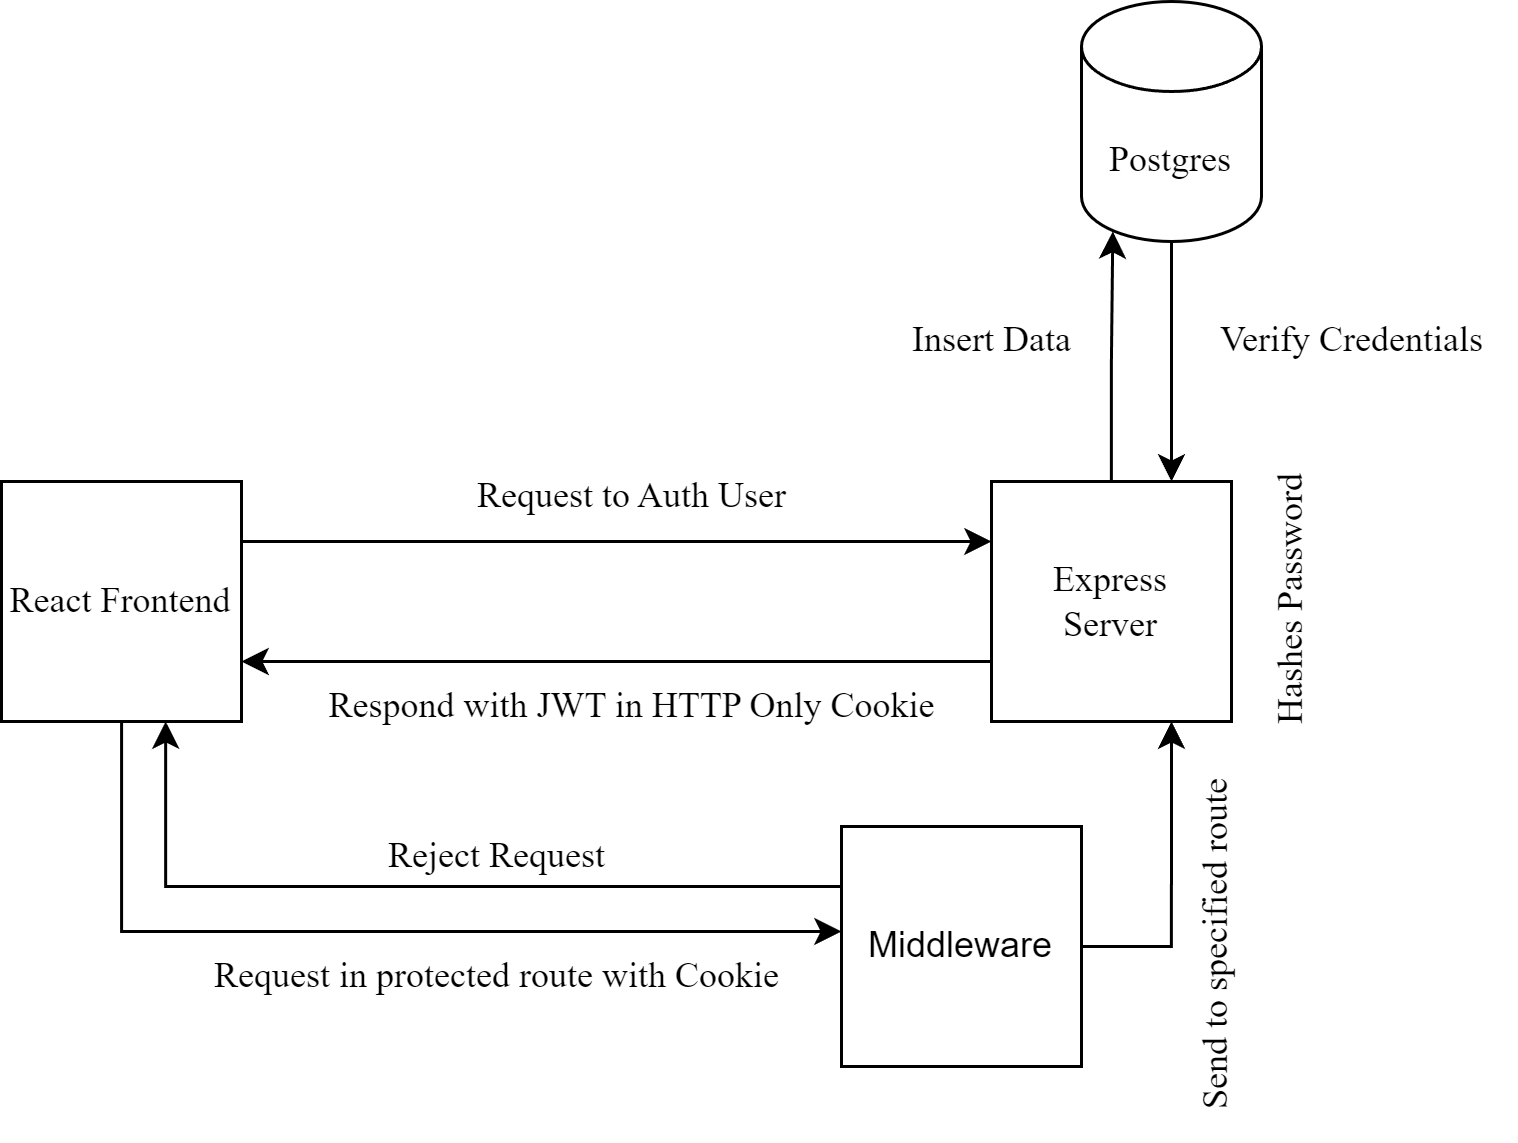
\includegraphics[height = 8cm]{Diagrams/auth module.png}
    \caption{Authentication Module}
\end{figure}
% \subsection{Algorithm Details}
% Here are some of the algorithms of our simulation models:

\subsection{Unit Testing Test Cases}
The following tables summarize the results of the main functions tests conducted on the application. Each test case is described along with the expected and actual outcomes to verify the functionality of the application. These results ensure that the application behaves as expected across various scenarios.

\begin{table}[h]
    \caption{Capsule Main Functions Testing}
    \label{tab:main_functions_testing}
    \resizebox{\textwidth}{!}{%
        \begin{tabular}{|c|p{1.5in}|p{3in}|p{3in}|p{0.5in}|}
            \hline
            \textbf{Test No.} & \textbf{Test Case} & \textbf{Expected Output} & \textbf{Actual Output} & \textbf{Result} \\
            \hline
            1 & Insert Capsule & Capsule object with ID and details is returned, including title, description, content, and associated simulations. & Capsule object with ID and details is returned, including title, description, content, and associated simulations. & Pass \\
            \hline
            2 & Read All Capsules & Array of capsule objects including \texttt{id}, \texttt{title}, \texttt{description}, and \texttt{thumbnail}, ordered by \texttt{id}. & Array of capsule objects including \texttt{id}, \texttt{title}, \texttt{description}, and \texttt{thumbnail}, ordered by \texttt{id}. & Pass \\
            \hline
            3 & Read Capsule By ID & Capsule details including simulation information for the specified ID, such as title, description, content, and associated simulation details. & Capsule details including simulation information for the specified ID, such as title, description, content, and associated simulation details. & Pass \\
            \hline
            4 & Update Capsule By ID & Success confirmation with updated capsule details reflecting changes in title, description, content, and linked simulations. & Success confirmation with updated capsule details reflecting changes in title, description, content, and linked simulations. & Pass \\
            \hline
            5 & Delete Capsule By ID & Success confirmation indicating the capsule with the specified ID has been deleted. & Success confirmation indicating the capsule with the specified ID has been deleted. & Pass \\
            \hline
            6 & Read Quiz By ID & Array of quiz details related to the specified capsule ID, including quiz questions and options. & Array of quiz details related to the specified capsule ID, including quiz questions and options. & Pass \\
            \hline
        \end{tabular}%
    }
\end{table}
\subsection{Test Cases for System Testing}
The objective of System Testing is to conduct a comprehensive evaluation of the entire PERN application, encompassing both frontend and backend components. This testing phase aims to validate the correct and cohesive functioning of all integrated parts of the system.
\\
\\
\textbf{General System Test Cases}\\
The following table summarizes the results of testing various general functionalities of the system/application. Each test case is designed to verify a specific functionality, including capsule access, category display, quiz operations, and simulator interactions. The table lists the test case number, description, input used, expected results, actual results obtained, and the outcome of the test. All tests have been successfully executed with the expected results matching the actual outcomes.
\begin{table}[H]
    \caption{General System Test Cases}
    \label{tab:general_functionalities_testing}
    \resizebox{\textwidth}{!}{%
        \begin{tabular}{|p{0.25in}|p{2in}|p{1.5in}|p{2.5in}|p{2in}|p{0.5in}|}
            \hline
            \textbf{Test No.} & \textbf{Test Case} & \textbf{Input} & \textbf{Expected Results} & \textbf{Actual Results} & \textbf{Result} \\
            \hline
            1 & Accessing Specific Capsules & 
            Capsule ID: 8 & 
            Shows the whole capsule, its images, PDF, and all its meta information with quiz. & 
            Shows the whole capsule, its images, PDF, and all its meta information with quiz. & 
            Pass \\
            \hline
            2 & Capsules By Category & 
            Category: Physics & 
            Shows cards, thumbnail, title, description, and buttons about related category capsules. & 
            Shows cards, thumbnail, title, description, and buttons about related category capsules. & 
            Pass \\
            \hline
            3 & Accessing Learning Areas & 
            Learning Area View & 
            Shows Learning Capsules with categories of each capsule. & 
            Shows Learning Capsules with categories of each capsule. & 
            Pass \\
            \hline
            4 & Accessing Quiz & 
            Quiz ID: 8 & 
            Shows Quiz of Specific Capsule. & 
            Shows Quiz of Specific Capsule. & 
            Pass \\
            \hline
            5 & Submitting Quiz & 
            Selected Quiz & 
            Shows how many quizzes were correct. & 
            Shows how many quizzes were correct. & 
            Pass \\
            \hline
            6 & Accessing Ohm's Law Simulator & 
            Simulator: Ohm's Law & 
            Shows Ohm's law simulator with V, I, and R inputs and phaser output. & 
            Shows Ohm's law simulator with V, I, and R inputs and phaser output. & 
            Pass \\
            \hline
            7 & Accessing PDF & 
            Open PDF Button & 
            Shows PDF document of specific capsule. & 
            Shows PDF document of specific capsule. & 
            Pass \\
            \hline
            8 & Accessing Images of Capsule & 
            Click Images Button & 
            Shows images related to capsule. & 
            Shows images related to capsule. & 
            Pass \\
            \hline
            9 & Searching Capsules and Simulations & 
            Search Term: Gravity & 
            Searches and shows capsules and simulations related to the search term. & 
            Searches and shows capsules and simulations related to the search term. & 
            Pass \\
            \hline
        \end{tabular}%
    }
\end{table}
\vspace{-1em}
\textbf{Authentication Unit Test Cases}\\
The following table presents the results of the authentication testing for the system/application. Each test case is aimed at verifying different authentication functionalities, including user and admin login, as well as user registration. The table provides details on the test case number, the specific test being performed, the input provided, the expected results, the actual results obtained, and the outcome of each test. All tests have been executed successfully, with results meeting the expected outcomes.
\begin{table}[H]
    \caption{Authentication Unit Test Cases}
    \resizebox{\textwidth}{!}{%
        \begin{tabular}{|p{0.20in}|p{1in}|p{2.25in}|p{2in}|p{2in}|p{0.5in}|}
            \hline
            \textbf{SN.} & \textbf{Test Case} & \textbf{Input} & \textbf{Expected Results} & \textbf{Actual Results} & \textbf{Result} \\
            \hline
            1 & Login User & 
            Username: 'sushantbram' \newline
            Password: 'sushant123' & 
            Logs in the User and shows profile & 
            Logs in the User and shows profile & 
            Pass \\
            \hline
            2 & Login Admin & 
            Username: 'Admin' \newline
            Password: 'labxplorerxadmin' & 
            Logs in Admin and shows profile & 
            Logs in Admin and shows profile & 
            Pass \\
            \hline
            3 & Login User with incorrect credentials & 
            Username: 'test' \newline
            Password: 'test1234' & 
            Alerts with wrong password & 
            Alerts with wrong password & 
            Pass \\
            \hline
            4 & Register User & 
            Username: 'Admin' \newline
            Password: 'admin' & 
            Registers User and shows profile & 
            Registers User and shows profile & 
            Pass \\
            \hline
        \end{tabular}%
    }
\end{table}
\vspace{-1em}
\textbf{Admin Functionalities  Test Cases}\\
The table below outlines the results of the admin functionalities testing for the system/application. This testing encompasses key administrative operations such as adding, editing, and deleting capsules, as well as managing quizzes. Each test case details the specific functionality being evaluated, the input provided, the expected results, the actual results obtained, and the final outcome of each test. All tests have been completed successfully, confirming that the admin functionalities operate as expected.

\begin{table}[H]
    \caption{Admin Functionalities Test Cases}
    \label{tab:admin_functionalities_testing}
    \resizebox{\textwidth}{!}{%
        \begin{tabular}{|p{0.25in}|p{1in}|p{2.5in}|p{2.5in}|p{2in}|p{0.5in}|}
            \hline
            \textbf{Test No.} & \textbf{Test Case} & \textbf{Input} & \textbf{Expected Results} & \textbf{Actual Results} & \textbf{Result} \\
            \hline
            1 & Add capsule & 
            Accessing Add Capsule Form & 
            Shows Form to add capsules and adds capsules when submitted & 
            Shows Form to add capsules and adds capsules when submitted & 
            Pass \\
            \hline
            2 & Edit capsule & 
            Accessing Edit Capsule Form for ID 6 & 
            Shows Form to edit capsules and updates capsule when submitted & 
            Shows Form to edit capsules and updates capsule when submitted & 
            Pass \\
            \hline
            3 & Delete capsule & 
            Deleting Capsule & 
            Deletes the selected capsule and confirms deletion & 
            Deletes the selected capsule and confirms deletion & 
            Pass \\
            \hline
            4 & Edit Quiz & 
            Accessing Quiz Management Form for ID 6 & 
            Shows Form to add quiz, remove quiz, and update options & 
            Shows Form to add quiz, remove quiz, and update options & 
            Pass \\
            \hline
        \end{tabular}%
    }
\end{table}
\vspace{-1em}
\textbf{User Functionalities Test Cases}\\
The following table presents the results of the user functionalities testing for the system/application. This testing evaluates crucial features available to users, including the ability to add items to favorites, comment on capsules, and view their profiles. Each test case details the specific functionality being tested, the input used, the expected outcomes, the actual results obtained, and the final result. All tests have been successfully passed, confirming that user functionalities are working as intended.

\begin{table}[H]
    \caption{User Functionalities Test Cases}
    \resizebox{\textwidth}{!}{%
        \begin{tabular}{|p{0.2in}|p{1.5in}|p{2.5in}|p{2in}|p{2in}|p{0.5in}|}
            \hline
            \textbf{SN.} & \textbf{Test Case} & \textbf{Input} & \textbf{Expected Results} & \textbf{Actual Results} & \textbf{Result} \\
            \hline
            1 & Favourite Function & 
            Clicking Add to Favourites button & 
            Adds to favourite and shows in profile & 
            Adds to favourite and shows in profile & 
            Pass \\
            \hline
            2 & Commenting & 
            Commenting on Capsules with "Good Capsule" & 
            Adds Comment and shows good capsule in both capsule and author profile & 
            Adds Comment and shows good capsule in both capsule and author profile & 
            Pass \\
            \hline
            3 & User Profile & 
            Viewing user profile & 
            Shows Profile having Favourite Capsule and Comments done by User & 
            Shows Profile having Favourite Capsule and Comments done by User & 
            Pass \\
            \hline
        \end{tabular}%
    }
\end{table}